\documentclass[portrait,a0]{a0poster}
%\documentclass[portrait,a0,posterdraft]{a0poster}
%
%
%
\usepackage[utf8]{inputenc}
\usepackage{tikz}
\usetikzlibrary{positioning}
\renewcommand{\familydefault}{\sfdefault} % use sans-serif font
\usepackage{sfmath} % use sans-serif math font
\usepackage{anyfontsize}
\usepackage{amsmath}
\usepackage{amsfonts}
\usepackage{amssymb}
\usepackage{natbib}
\usepackage{yfonts}
\usepackage{stmaryrd}
\usepackage{float}
\usepackage{amsthm}
\usepackage{thmtools}
\usepackage{enumitem}
\DeclareMathOperator*{\argmin}{arg\,min}
%
%
%
%
%
%
% ADDITIONAL USEPACKAGES
%
\usepackage{dsfont}
%
%
%
% TITLE
\def\myTitle{Frequentist analysis of Bayesian methods for statistical ill-posed inverse problems}
%
% NAME
\def\myName{Xavier Loizeau}
%
% SUPERVISORS
\def\mySuperv{Prof. Dr. Jan Johannes, Prof. Dr. Claudia Schillings}
%
%
%
% PERSONAL MACROS
%
\def\content{% dummy content
	Lorem ipsum dolor sit amet, consetetur sadipscing elitr, sed diam nonumy eirmod tempor invidunt ut labore et dolore magna aliquyam erat, sed diam voluptua. At vero eos et accusam et justo duo dolores et ea rebum. Stet clita kasd gubergren, no sea takimata sanctus est Lorem ipsum dolor sit amet. Lorem ipsum dolor sit amet, consetetur sadipscing elitr, sed diam nonumy eirmod tempor invidunt ut labore et dolore magna aliquyam erat, sed diam voluptua. At vero eos et accusam et justo duo dolores et ea rebum. Stet clita kasd gubergren, no sea takimata sanctus est Lorem ipsum dolor sit amet.%
}
%
%
%
%
%
%
% LENGTHS
%
\newlength{\myTopToPretitleVSpace}
\setlength{\myTopToPretitleVSpace}{0mm}
\newlength{\myPreTitleInnerYSep}
\setlength{\myPreTitleInnerYSep}{15mm}
\newlength{\preTitleSpaceLength}
\setlength{\preTitleSpaceLength}{8mm}
\newlength{\myMainTitleInnerYSep}
\setlength{\myMainTitleInnerYSep}{15mm}
\newlength{\myMainTitleFooterHeight}
\setlength{\myMainTitleFooterHeight}{5mm}
\newlength{\myMainTitleToBodyVSpace}
\setlength{\myMainTitleToBodyVSpace}{25mm}
\newlength{\myFooterHeaderHeight}
\setlength{\myFooterHeaderHeight}{5mm}
\newlength{\myFooterBodyInnerYSep}
\setlength{\myFooterBodyInnerYSep}{10mm}
\newlength{\myFooterBodyColumnSize}
\setlength{\myFooterBodyColumnSize}{400mm}
\newlength{\myBlockColHSpace}
\setlength{\myBlockColHSpace}{15mm}
\newlength{\myBlockToBlockVSpace}
\setlength{\myBlockToBlockVSpace}{15mm}
\newlength{\myBlockTitleToBodyVSpace}
\setlength{\myBlockTitleToBodyVSpace}{0mm}
\newlength{\myBlockInnerXSep}
\setlength{\myBlockInnerXSep}{0mm}
\newlength{\myBlockInnerYSep}
\setlength{\myBlockInnerYSep}{0mm}
\newlength{\myBlockBodyInnerXSep}
\setlength{\myBlockBodyInnerXSep}{10mm}
\newlength{\myBlockBodyInnerYSep}
\setlength{\myBlockBodyInnerYSep}{10mm}
\newlength{\myBlockTextWidth}
\setlength{\myBlockTextWidth}{385mm}
%
%
%
% COLORS
%
\definecolor{colorBg}{HTML}{FFFFFF}
\definecolor{RTGblue}{HTML}{003466}
\definecolor{RTGred}{HTML}{C80B33}
\definecolor{RTGgray}{HTML}{3C3C3C}
\definecolor{RTGlightgray}{HTML}{DCDCDC}
\colorlet{colMainBg}{RTGlightgray}
\colorlet{colPreTitleBg}{colorBg}
\colorlet{colPreTitleFg}{RTGgray}
\colorlet{colMainTitleBg}{RTGblue}
\colorlet{colMainTitleFg}{white}
\colorlet{colFooterBodyBg}{RTGblue}
\colorlet{colFooterBodyFg}{white}
\colorlet{colFooterHeaderBg}{RTGred}
\colorlet{colFooterHeaderFg}{white}
\colorlet{colBlockBg}{RTGlightgray}
\colorlet{colBlockFg}{black}
\colorlet{colBlockTitleBg}{RTGblue}
\colorlet{colBlockTitleFg}{white}
\colorlet{colBlockBodyBg}{white}
\colorlet{colBlockBodyFg}{RTGgray}
%
%
%
% FONT STYLE
%
% available font sizes:
%\tiny          12pt
%\scriptsize    14.4pt
%\footnotesize  17.28pt
%\small         20.74pt
%\normalsize    24.88pt
%\large         29.86pt
%\Large         35.83pt
%\LARGE         43pt
%\huge          51.6pt
%\Huge          61.92pt
%\veryHuge      74.3pt
%\VeryHuge      89.16pt
%\VERYHuge      107p
\newcommand*{\fsPreTitle}{\fontsize{74.3}{89}\selectfont\bf}
\newcommand*{\fsPreTitleRTG}{\LARGE\bf}
\newcommand*{\fsMainTitle}{\Huge}
\newcommand*{\fsName}{\LARGE\bf}
\newcommand*{\fsSuperv}{\LARGE}
\newcommand*{\fsBlockTitle}{\LARGE\bf}
\newcommand*{\fsBlockBody}{\normalsize}
\newcommand*{\fsFooterLeft}{\Large}
\newcommand*{\fsFooterRight}{\LARGE\bf}
%
%
%
% PRETITLE: a block for the pre-title at the very top
%
\newcommand{\myPreTitle}{%
	\vspace*{\myTopToPretitleVSpace}\\
	\begin{minipage}[c]{18cm}
		\centering
		
\includegraphics[height=5cm]{logoMAt} 
		%\includegraphics[height=7cm]{logoMA} 
	\end{minipage}
	\begin{minipage}[c]{40cm}%
		\centering%
		{\fsPreTitle%
		\spaceskip=0.25em
		Statistical Modeling of\\Complex Systems and Processes\par}
	\end{minipage}
	\hspace*{-1cm}
	\begin{minipage}[c]{18cm}
		\centering
		
\includegraphics[height=7cm]{logoHDt} 
		%\includegraphics[height=7cm]{logoHD} 
	\end{minipage}%
}
%
%
%
% MAINTITLE: a block for the title and name
%
\newcommand{\myMainTitle}{%
	
\begin{tikzpicture}[]
		\node[
			colMainTitleFg,
			fill=colMainTitleBg,
			anchor=north,
			align=center,
			inner xsep=0,
			inner ysep=\myMainTitleInnerYSep,
		] (mainTitleBody) {%
			{\fsMainTitle%
			\spaceskip=0.25em%
			\myTitle}%
			\\%
			\vspace*{10mm}%
			{\fsName%
			\spaceskip=0.25em%
			\myName}%
			\\%
			\vspace*{10mm}%
			{\fsSuperv%
				\spaceskip=0.25em%
				Supervisors: \mySuperv}%
		};
		\node[
			fill=RTGred,
			anchor=north,
			align=center,
			inner xsep=0,
			inner ysep=0,
			minimum height=\myMainTitleFooterHeight,
			below =0of mainTitleBody,
		] (mainTitleFooter) {};
	\end{tikzpicture}
}
%
%
%
% FOOTER: block at the very bottom of the poster
%
\newcommand{\myFooter}{%
	\begin{tikzpicture}[]
		\node[
			colFooterBodyFg,
			fill=colFooterBodyBg,
			anchor=south,
			align=center,
			inner xsep=0,
			inner ysep=\myFooterBodyInnerYSep,
		] (footerBody) {
			\begin{minipage}[c]{\myFooterBodyColumnSize}
				\fsFooterLeft
				Supported by\hspace{0.5em}
				
\includegraphics[height=15mm]{logoDFG}
			\end{minipage}
			\begin{minipage}[c]{\myFooterBodyColumnSize}
				\flushright
				\fsFooterRight
				RTG 1953
			\end{minipage}	
		};
		\node[
			colFooterHeaderFg,
			fill=colFooterHeaderBg,
			anchor=south,
			align=center,
			inner xsep=0,
			inner ysep=0,
			minimum height=\myFooterHeaderHeight,
			above =0of footerBody,
		] (footerHeader) {};
	\end{tikzpicture}
}
%
%
%
% INNERBLOCK: Content of a Block: BlockTitle, BlockBody
%
\newcommand{\myInnerBlock}[2]{%
	\begin{tikzpicture}[]
	\ifx&#1&
	\node[
	colBlockBodyFg,
	fill=colBlockBodyBg,
	anchor=center,
	align=justify,
	inner xsep=\myBlockBodyInnerXSep,
	inner ysep=\myBlockBodyInnerYSep,
	text width=\myBlockTextWidth-2.*\myBlockInnerXSep-2.*\myBlockBodyInnerXSep,
	] (body) {%
		\fsBlockBody%
		#2%
		\par%
	};
	\else
	\node[
	colBlockTitleFg,
	fill=colBlockTitleBg,
	anchor=center,
	align=center,
	inner xsep=\myBlockBodyInnerXSep,
	inner ysep=0mm,
	text width=\myBlockTextWidth-2.*\myBlockInnerXSep-2.*\myBlockBodyInnerXSep,
	] (title) at (0,0) {%
		\vspace*{12mm}%
		\\%
		\fsBlockTitle%
		\spaceskip=0.25em
		#1%
		\vspace*{10mm}%
	};
	\node[
	colBlockBodyFg,
	fill=colBlockBodyBg,
	anchor=center,
	align=justify,
	inner xsep=\myBlockBodyInnerXSep,
	inner ysep=\myBlockBodyInnerYSep,
	text width=\myBlockTextWidth-2.*\myBlockInnerXSep-2.*\myBlockBodyInnerXSep,
	below =\myBlockTitleToBodyVSpace of title
	] (body) {%
		\fsBlockBody%
		#2%
		\par%
	};
	\fi
	\end{tikzpicture}
}
%
%
%
% BLOCKSTYLE: style for blocks, which surround BlockTitle and BlockBody
%
\tikzset{BlockStyle/.style={%
		colBlockFg,
		fill=colBlockBg,
		anchor=north west,
		inner sep=0,
		rectangle, 
		text width=\myBlockTextWidth-2.*\myBlockInnerXSep,
		inner xsep=\myBlockInnerXSep,
		inner ysep=\myBlockInnerYSep,
	}
}
%
%
%
% BLOCK: command for placing a new block below the previous one
%
\newcounter{myColumnCounter}
\newcounter{myBlockCounter}[myColumnCounter]
%
\newcommand{\myFirstBlock}[2]{%
	\node[%
		BlockStyle,
	] (a) {%
		\myInnerBlock{#1}{#2}%
	};%
}%
%
\newcommand{\myFurtherBlock}[2]{%
	\node[%
		BlockStyle,
		below =\myBlockToBlockVSpace of a,
	] (a) {%
		\myInnerBlock{#1}{#2}%
	};%
}%
%
\newcommand{\myBlock}[2]{%
	\ifnum\themyBlockCounter=0%
		\myFirstBlock{#1}{#2}%
	\else%
		\myFurtherBlock{#1}{#2}%
	\fi%
	\stepcounter{myBlockCounter}%
}
%
%
%
% THEOREM STYLES
%
\declaretheoremstyle[
	bodyfont=\normalfont,
	postfoothook={\vspace*{30pt}},
	preheadhook={},
	mdframed={
		backgroundcolor = RTGlightgray!40!white,
		innertopmargin = 20pt,
		innerbottommargin = 20pt,
		innerrightmargin = 20pt,
		innerleftmargin = 20pt,
		skipabove = 30pt,
		skipbelow = 30pt,
		leftmargin = 30pt,
		rightmargin = 30pt,
		%		roundcorner = 0pt,
		%		topline = true,
		%		bottomline = true,
		leftline = false,
		rightline = false,
		%		hidealllines = true,
		linewidth = 5pt,
		%		innerlinewidth = 5pt,
		%		middlelinewidth = 6pt,	
		%		outerlinewidth = 2pt,
		linecolor = RTGred,
		%		innerlinecolor = orange,
		%		middlelinecolor = green,	
		%		outerlinecolor = RTGblue,
		%		fontcolor = black,
		%		font = ?,
		%		shadow = true,
		%		shadowsize = 8pt,
		%		shadowcolor = black!50,
		%		frametitle = {Title},
		%		frametitle<Option...>,
		%		%\mdfsubtitle{SubTitle}
		%		subtitle<Option...>,
		%		tikzsetting = {},
		%		align =center,
		%		extra = {},		
	}]{redHLineStyle}
%
%
% numbered
\declaretheorem[style=redHLineStyle,name=Definition]{definition}
\declaretheorem[style=redHLineStyle,name=Lemma,numberlike=definition]{lemma}
\declaretheorem[style=redHLineStyle,name=Theorem,numberlike=definition]{theorem}
\declaretheorem[style=redHLineStyle,name=Corollary,numberlike=definition]{corollary}
\declaretheorem[style=redHLineStyle,name=Remark,numberlike=definition]{remark}
\declaretheorem[style=redHLineStyle,name=Example,numberlike=definition]{example}
%
% no numbering
\declaretheorem[style=redHLineStyle,name=Definition,numbered=no]{definition*}
\declaretheorem[style=redHLineStyle,name=Lemma,numbered=no]{lemma*}
\declaretheorem[style=redHLineStyle,name=Theorem,numbered=no]{theorem*}
\declaretheorem[style=redHLineStyle,name=Corollary,numbered=no]{corollary*}
\declaretheorem[style=redHLineStyle,name=Remark,numbered=no]{remark*}
\declaretheorem[style=redHLineStyle,name=Example,numbered=no]{example*}
%
%
%
%
%
%
%
\begin{document}
%
	\thispagestyle{empty}
	%
	\begin{tikzpicture}[remember picture, overlay]
	%
	% BACKGROUND
		\fill[
			colMainBg, 
			inner sep=0pt, 
			line width=0pt
		] (current page.north east) rectangle (current page.south west); 
	%
	% PRE-TITLE
		\node[
			colPreTitleFg, 
			fill=colPreTitleBg,
			anchor=north,
			align=center,
			inner xsep=0,
			inner ysep=\myPreTitleInnerYSep,
			text width=\paperwidth
		] (pretitle) at (current page.north) {
			\myPreTitle
		};
	%
	% MAIN TITLE
		\node[
			anchor=north,
			align=center,
			below=0of pretitle,
			inner xsep=0,
			inner ysep=0,
			text width=\paperwidth
		] (maintitle) {
			\myMainTitle
		};
	%
	% FOOTER
		\node[
			anchor=south,
			align=center,
			inner xsep=0,
			inner ysep=0,
			text width=\paperwidth
		]  (footer) at (current page.south) {
	 		\myFooter
		};
	%
	% BODY
		\matrix[
			inner sep=0, 
			column sep=\myBlockColHSpace, 
			row sep=0cm,
			below=\myMainTitleToBodyVSpace of maintitle,
			ampersand replacement=\&,
		] (m) {
			\stepcounter{myColumnCounter};
			%
%
%
%%%%%%%%%%%%%%%%%%%%%%%%%%%%%%%%%%%%%%%%%%%%%%%%%%%%%%%%%%%%%%%%%%%%%%%%%%%%%%%%
% BEGIN LEFT COLUMN
%%%%%%%%%%%%%%%%%%%%%%%%%%%%%%%%%%%%%%%%%%%%%%%%%%%%%%%%%%%%%%%%%%%%%%%%%%%%%%%%
%
%
%
\myBlock{The inverse Gaussian sequence space model}{%
Consider an indirect Gaussian sequence space model consisting of:
\begin{itemize}
\item an unknown parameter of interest $\left(\theta^{\circ}_{j}\right)_{j \in \mathbb{N}} = \theta^{\circ}$,
\item a decreasing multiplicative sequence $\left(\lambda_{j}\right)_{j \in \mathbb{N}} = \lambda$ converging to $0$,
\item observations $\left(Y_{j}\right)_{j \in \mathbb{N}} = Y$, contaminated by an additive independent centered Gaussian noise with variance $n^{-1}, \quad Y = \left(\theta^{\circ}_{j} \cdot \lambda_{j} + \sqrt{n}^{-1} \cdot \xi_{j}\right)_{j \in \mathbb{N}}, \quad \left(\xi_{j}\right)_{j \in \mathbb{N}} \sim_{iid} \mathcal{N}\left(0, 1\right).$
\end{itemize}

The goal is to recover $\theta^{\circ}$ and derive an upper bound.
}%
%
%
%\myBlock{The frequentist model selection}{%
%For any index $j$, an unbiased estimator of $\theta^{\circ}_{j}$ is $Y_{j}/\lambda_{j}$.
%Hence, an intuitive class of estimators are the projection estimators: $\tilde{\theta}^{m} = \left(Y_{j}/\lambda_{j} \mathds{1}_{\left\{j \leq m\right\}}\right)_{j \in \mathbb{N}}$ with $m$ in $\mathbb{N}$.
%The model selection method offers a data driven way to select $m$ in this context:
%
%\textcolor{red!90!black}{
%\begin{alignat*}{3}
%&G_{n} && := \max\left\{1 \leq j \leq n : n^{-1} \lambda_{j}^{-2} \leq \lambda_{1}^{-2}\right\}, &&\\
%&\widehat{m} && := \argmin\limits_{m \in \left\llbracket 1 , G_{n} \right\rrbracket}\left\{3 m -\sum\limits_{j = 1}^{m} Y_{j}^{2}\right\}, &&\widehat{\theta} := \left( \tilde{\theta}^{\widehat{m}}_{j} \right)_{j \in \mathbb{N}}.
%\end{alignat*}}
%
%\bigskip
%
%It is shown in \citet{PM}, in the direct case, that this estimator is \textcolor{red!90!black}{consistent}, converges in probability and $\mathbb{L}^{2}$-norm, noted $\Vert \cdot \Vert$, with \textcolor{red!90!black}{minimax optimal rate} over some Sobolev ellipsoid:
%\[\textcolor{red}{\Theta^{\circ} := \Theta^{\circ}\left(\textgoth{a}, L^{\circ}\right) \left\{\theta : \sum\limits_{j = 1}^{\infty} \frac{1}{\textgoth{a}_{j}}\theta_{j}^{2} < L^{\circ}\right\}}.\]
%}%
%%
%%
\myBlock{Bayesian paradigm}{%
We adopt a \textcolor{red!90!black}{Bayesian point of view}:
\begin{itemize}
\item the parameter $\boldsymbol{\theta}$ is a random variable with prior $\mathbb{P}_{\boldsymbol{\theta}},$
\item given $\boldsymbol{\theta}$, the likelihood of $Y$ is $\mathbb{P}_{Y \vert \boldsymbol{\theta}}^{n} = \mathcal{N}\left(\boldsymbol{\theta} \lambda, n^{-1} \mathbb{I}\right),$
\item we are interested in the posterior distribution $\mathbb{P}_{\boldsymbol{\theta} \vert Y}^{n} \propto \mathbb{P}_{Y \vert \boldsymbol{\theta}}^{n} \cdot \mathbb{P}_{\boldsymbol{\theta}}.$
\end{itemize}

\bigskip

Within this framework we define the estimator: $\textcolor{red!90!black}{\widehat{\theta} := \mathbb{E}_{\boldsymbol{\theta}\vert Y}^{n}\left[\boldsymbol{\theta}\right]}.$

\medskip

We are interested in the behavior of $\mathbb{P}_{\boldsymbol{\theta}\vert Y}^{n}$ as $n$ tends to infinite.

\medskip

In particular, the question of oracle and minimax concentration (resp. convergence) is answered for the posterior distribution (resp. posterior mean).
}%
%
%
\myBlock{Hierarchical prior}{%
\begin{itemize}
\item Consider a \textcolor{red!90!black}{random hyper-parameter $M$}, with values in a subset of $\mathbb{N}$, acting like a threshold:

\[\forall j > m , \quad \mathbb{P}_{\boldsymbol{\theta}_{j}\vert M = m} = \delta_{0}, \quad \quad \forall j \leq m , \quad \mathbb{P}_{\boldsymbol{\theta}_{j}\vert M = m} = \mathcal{N}\left(0, 1\right).\]
\item If we denote $\mathbb{P}_{M}$ the distribution of $M$ (to be specified later), then
\[\textcolor{red!90!black}{\mathbb{P}_{\boldsymbol{\theta}\vert Y}^{n} = \sum\limits_{m \in \mathbb{N}} \mathbb{P}_{\boldsymbol{\theta} \vert M = m, Y}^{n} \cdot \mathbb{P}_{M = m \vert Y}^{n}}.\]
%\end{column}
%\begin{column}{.45\textwidth} % The second subdivided column within the first main column
%\begin{figure}
%\centering
% 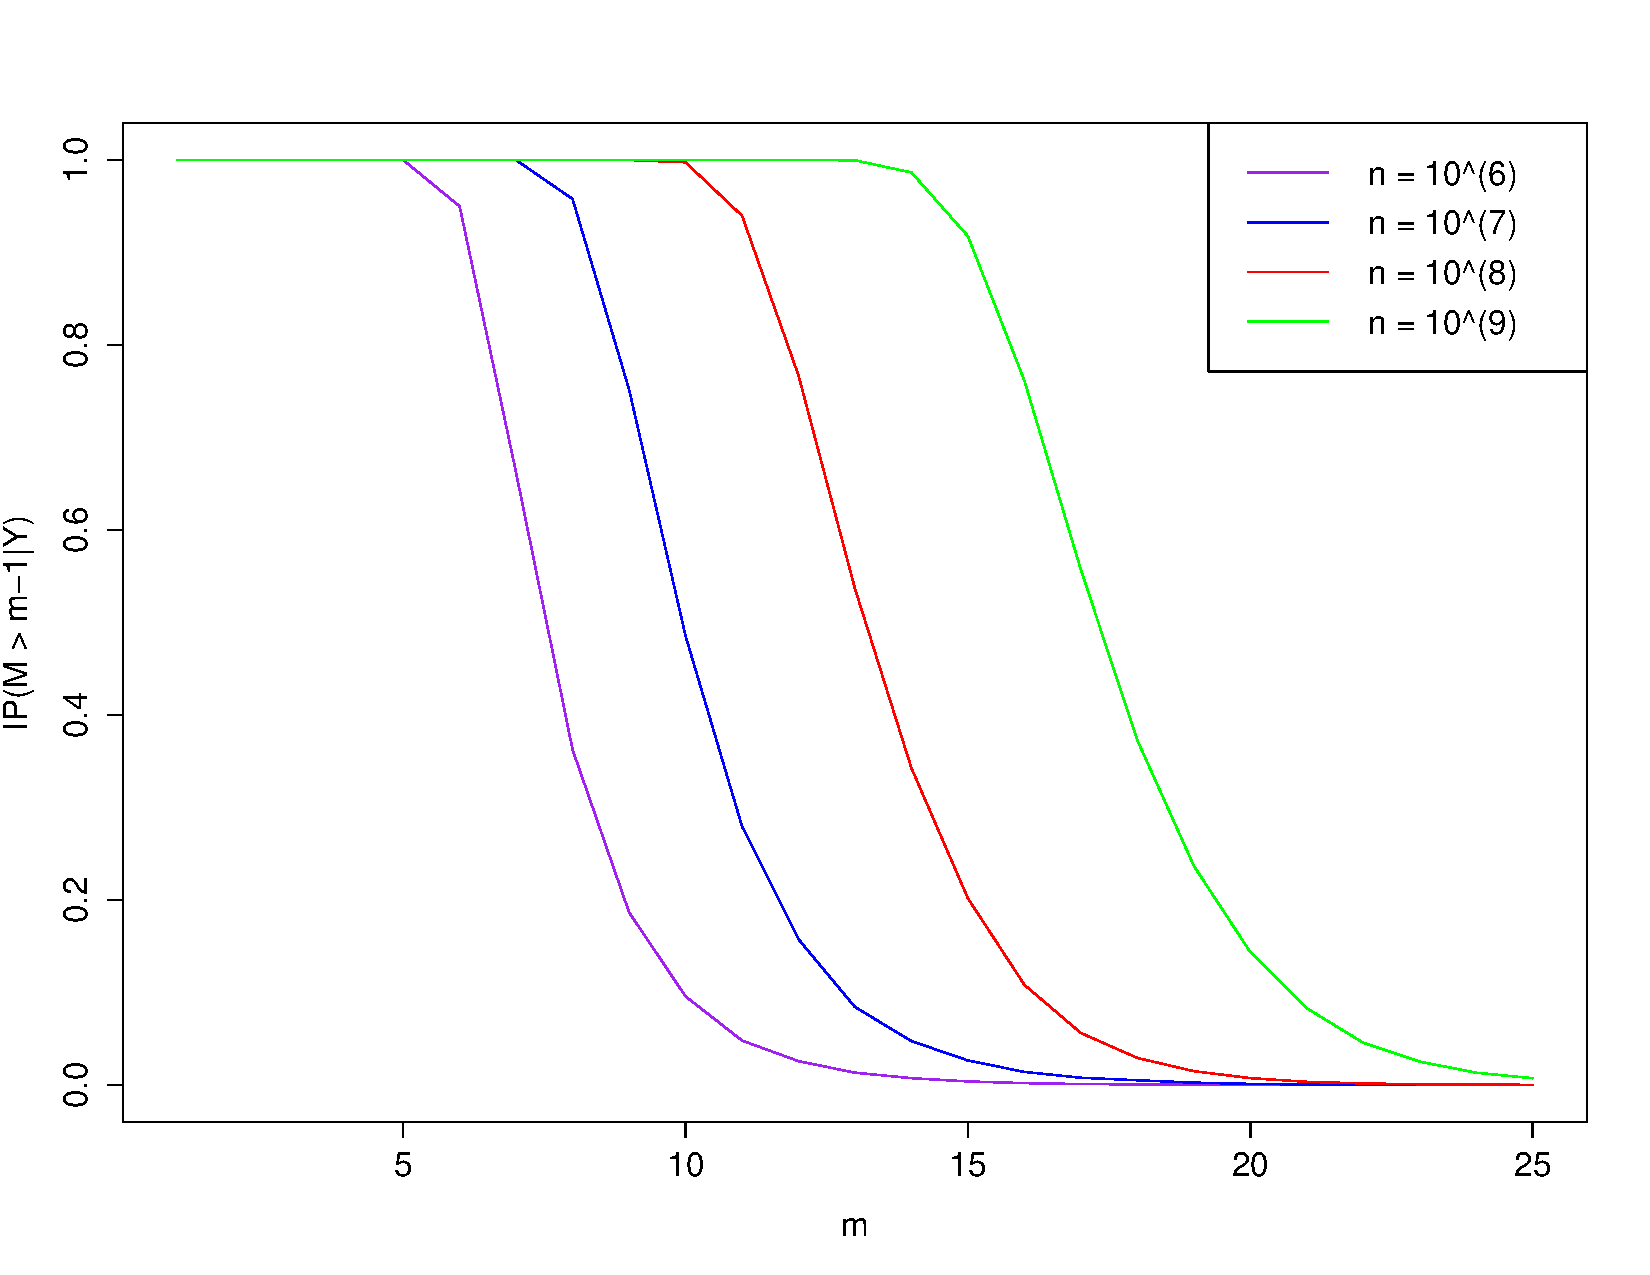
\includegraphics[width=1\linewidth]{M.pdf}
%\caption{Survival function of $M$ for different values of $n$}\label{M}
%\end{figure}
%\end{column}
%\end{columns} % End of the subdivision
\item Hence, given $M$, the posterior is
\begin{align*}
\forall j > m, &\quad \boldsymbol{\theta}_{j} \vert M = m, Y \sim \delta_{0},\\
\forall j \leq m, &\quad \boldsymbol{\theta}_{j} \vert M = m, Y \sim \mathcal{N}\left(\frac{Y_{j} \cdot n \cdot \lambda_{j}}{1 + n \cdot \lambda_{j}^{2}}, \frac{1}{1 + n \cdot \lambda_{j}^{2}} \right).
\end{align*}
\end{itemize}
\underline{Remark:} the family of hierarchical priors with deterministic threshold $M$ is called family of sieve priors.

%\begin{figure}[H]
%\centering
% 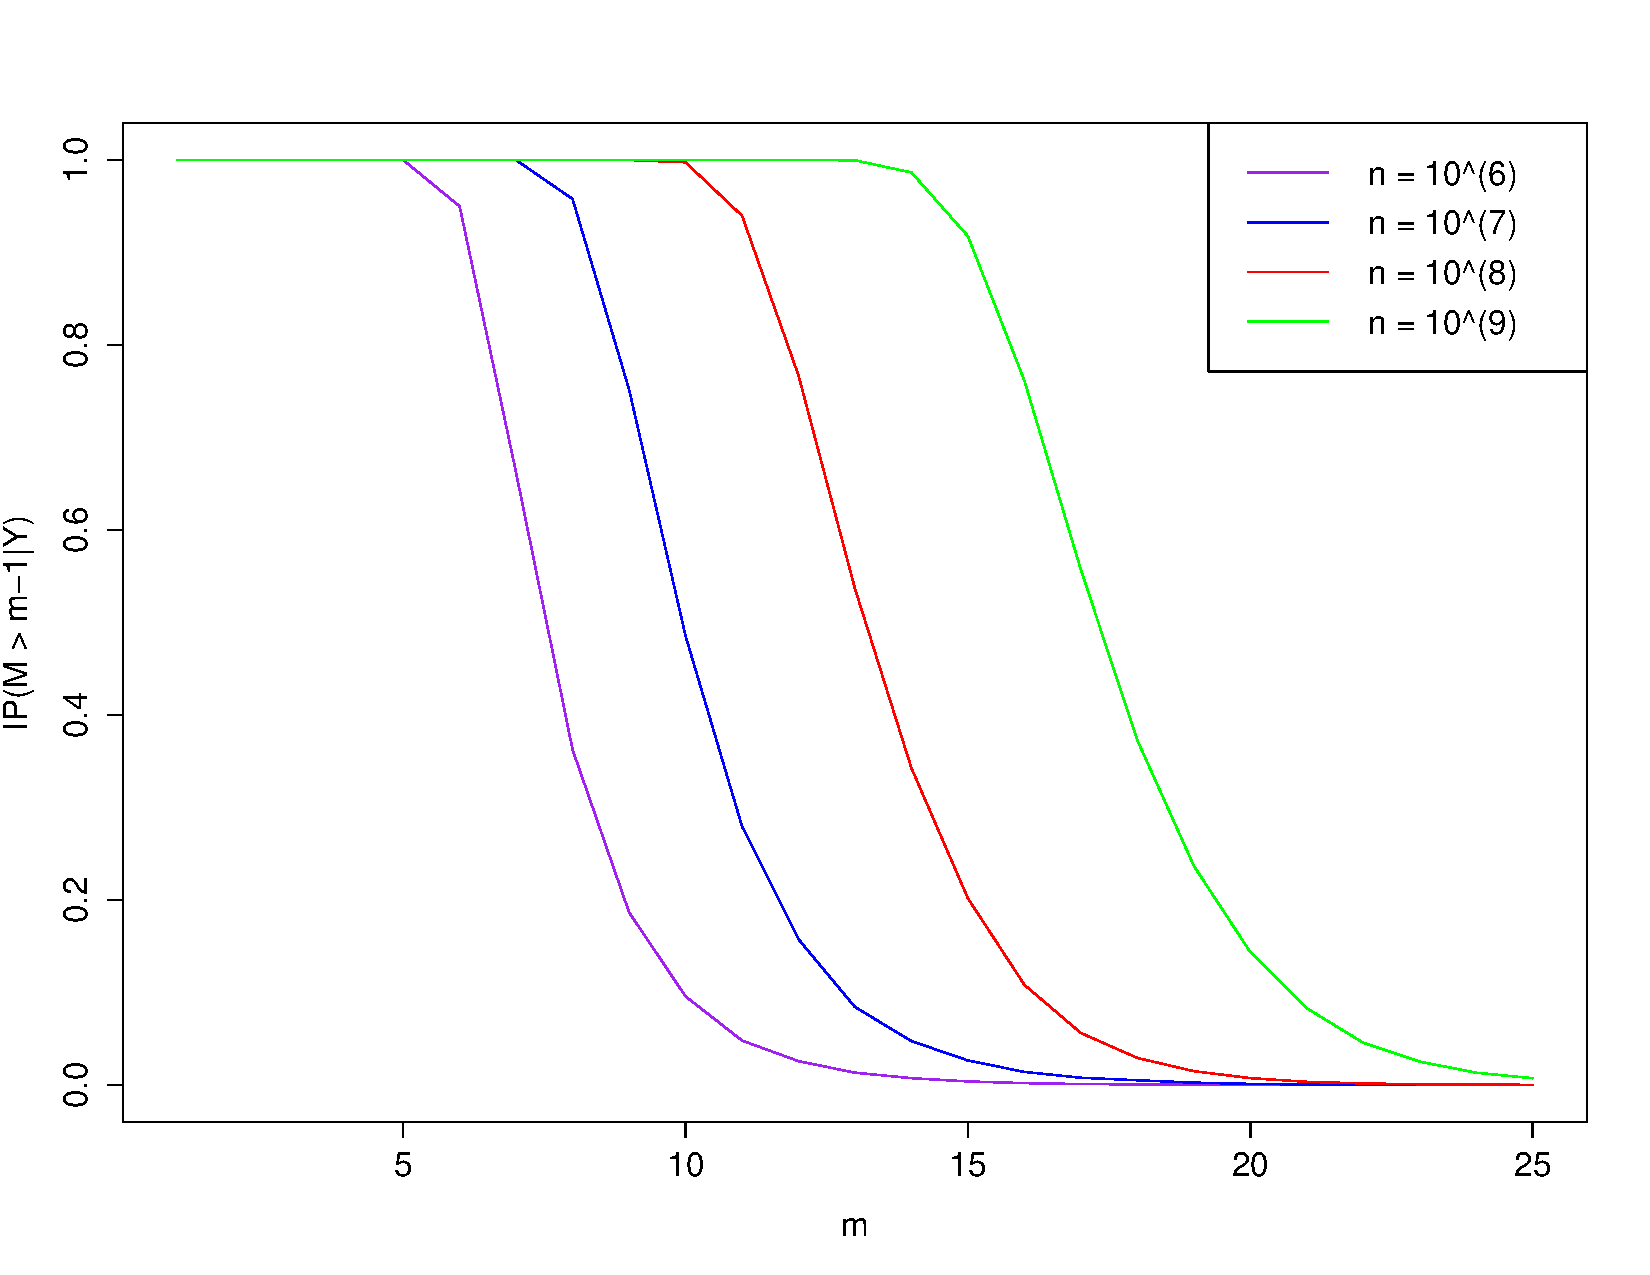
\includegraphics[width=0.4\linewidth]{M.pdf}
%\caption{Survival function of $M$ for different values of $n$}\label{M}
%\end{figure}
}%
%
%
\myBlock{Review : optimal posterior concentration}{%
	In \cite{JJASRS}, under a \textcolor{red!90!black}{pragmatic Bayesian} point of view; that is, the existence of a true parameter $\theta^{\circ}$ is accepted; it is shown that, by choosing $\mathbb{P}_{M}$ suitably:
\begin{itemize}
	\item the Bayes estimator $\widehat{\theta}$ \textcolor{red!90!black}{converges with,}
	\begin{itemize}
		\item \textcolor{red!90!black}{oracle optimal rate} for the quadratic risk which means, $\forall \theta^{\circ} \in \Theta^{\circ}, \exists C^{\circ} \in \left[ 1, \infty \right[ : \forall n \in \mathbb{N}, \exists \Phi_{n}^{\circ} \in \mathbb{R}:$
		\[\inf\limits_{m \in \mathbb{N}} \, \mathbb{E}_{\theta^{\circ}}^{n}\left[\left\Vert \tilde{\theta}^{m} - \theta^{\circ} \right\Vert^{2}\right] \geq \Phi_{n}^{\circ}(\theta^{\circ}), \quad \quad \mathbb{E}_{\theta^{\circ}}^{n}\left[\left\Vert \widehat{\theta} - \theta^{\circ} \right\Vert^{2}\right] \leq C^{\circ} \Phi_{n}^{\circ}(\theta^{\circ});\]
		\item \textcolor{red!90!black}{minimax optimal rate} for the maximal risk over some ellipsoid $\Theta^{\circ}_{a}$, that is to say, $\exists C^{\star} \in \left[ 1, \infty \right[ : \forall n \in \mathbb{N}, \exists \Phi_{n}^{\star}(a) \in \mathbb{R}:$
\[\inf\limits_{\tilde{\theta}} \sup\limits_{\theta^{\circ} \in \Theta^{\circ}_{a}} \mathbb{E}_{\theta^{\circ}}^{n}\left[\left\Vert \tilde{\theta} - \theta^{\circ} \right\Vert^{2}\right] \geq \Phi_{n}^{\star}(a), \quad \quad \sup\limits_{\theta^{\circ} \in \Theta^{\circ}_{a}} \mathbb{E}_{\theta^{\circ}}^{n}\left[\left\Vert \widehat{\theta} - \theta^{\circ} \right\Vert^{2}\right] \leq C^{\star} \Phi_{n}^{\star}(a),\]
where $\inf\limits_{\tilde{\theta}}$ is taken over all possible estimators of $\theta^{\circ}$;
	\end{itemize}
	\item the posterior distribution \textcolor{red!90!black}{concentrates with,}
	\begin{itemize}
		\item \textcolor{red!90!black}{oracle optimal rate} for the quadratic loss which means, $\forall \theta^{\circ} \in \Theta^{\circ}, \exists K^{\circ} \in \left[ 1, \infty \right[ :$
\[\lim\limits_{n \rightarrow \infty} \mathbb{E}_{\theta^{\circ}}^{n}\left[\mathbb{P}_{\boldsymbol{\theta}\vert Y}^{n}\left(\left\Vert \boldsymbol{\theta} - \theta^{\circ} \right\Vert^{2} \leq K^{\circ} \Phi_{n}^{\circ}\right)\right] = 1;\]
		\item \textcolor{red!90!black}{minimax optimal rate over $\Theta^{\circ}_{a}$}, that is to say, for any unbounded sequence $K_{n} \in \mathbb{R}^{\mathbb{N}} :$
\[\lim\limits_{n \rightarrow \infty} \sup\limits_{\theta^{\circ} \in \Theta^{\circ}_{a}}  \mathbb{E}_{\theta^{\circ}}^{n}\left[\mathbb{P}_{\boldsymbol{\theta}\vert Y}^{n}\left(\left\Vert \boldsymbol{\theta} - \theta^{\circ} \right\Vert^{2} \leq K_{n} \Phi_{n}^{\star}(a)\right)\right] = 1.\]
	\end{itemize}
\end{itemize}
}%
%
%
%
%
%%%%%%%%%%%%%%%%%%%%%%%%%%%%%%%%%%%%%%%%%%%%%%%%%%%%%%%%%%%%%%%%%%%%%%%%%%%%%%%%
% END LEFT COLUMN
%%%%%%%%%%%%%%%%%%%%%%%%%%%%%%%%%%%%%%%%%%%%%%%%%%%%%%%%%%%%%%%%%%%%%%%%%%%%%%%%
%
%
%
\& \stepcounter{myColumnCounter}; % Do not change.
%
%
%
%%%%%%%%%%%%%%%%%%%%%%%%%%%%%%%%%%%%%%%%%%%%%%%%%%%%%%%%%%%%%%%%%%%%%%%%%%%%%%%%
% BEGIN RIGHT COLUMN
%%%%%%%%%%%%%%%%%%%%%%%%%%%%%%%%%%%%%%%%%%%%%%%%%%%%%%%%%%%%%%%%%%%%%%%%%%%%%%%%
%
%
%
\myBlock{Bayesian formulation of optimality}{%
\begin{theorem}
	For all $\theta^{\circ}$ in $\Theta^{\circ},$ 
	
	\[\lim\nolimits_{n \rightarrow \infty} \inf\nolimits_{\mathbb{Q}_{\boldsymbol{\theta}}}\, \mathbb{E}_{\theta^{\circ}}^{n}\left[\mathbb{Q}_{\boldsymbol{\theta} \vert Y}^{n}\left(\left\Vert \boldsymbol{\theta} - \theta^{\circ} \right\Vert^{2} \geq \Phi_{n}^{\circ}\right)\right] = 1,\]

	where $\inf_{\mathbb{Q}_{\boldsymbol{\theta}}}$ is taken over all sieve priors; \textcolor{red!90!black}{establishing a Bayesian formulation of oracle optimality}.
\end{theorem}
\vspace{-1cm}
\begin{theorem}
	We also have, for some Sobolev's ellipsoids $\Theta^{\circ}_{a},$
	
	\vspace{-1cm}
	
	\[\lim\nolimits_{n \rightarrow \infty} \inf\nolimits_{\mathbb{Q}_{\boldsymbol{\theta}}}\sup\nolimits_{\theta^{\circ} \in \Theta^{\circ}_{a}}\, \mathbb{E}_{\theta^{\circ}}^{n}\left[\mathbb{Q}_{\boldsymbol{\theta} \vert Y}^{n}\left(\left\Vert \boldsymbol{\theta} - \theta^{\circ} \right\Vert^{2} \geq \Phi_{n}^{\star}(a)\right)\right] = 1,\]
	
	\vspace{-0.5cm}
	
	where $\inf_{\mathbb{Q}_{\boldsymbol{\theta}}}$ is taken over all possible sieve priors.

\end{theorem}
}

\myBlock{Iterated posterior}{
In the spirit of \cite{OBJJ}, we then generate a posterior family by introducing an \textcolor{red!90!black}{iteration parameter $\eta$}:
\begin{itemize}
\item for $\eta = 1$, the prior distribution is $\mathbb{P}_{\boldsymbol{\theta}^{1}} = \mathbb{P}_{\boldsymbol{\theta}}$, the likelihood $\mathbb{P}_{Y^{1} \vert \boldsymbol{\theta}^{1}}^{n} = \mathbb{P}_{Y \vert \boldsymbol{\theta}}^{n}$ and the posterior distribution is $\mathbb{P}_{\boldsymbol{\theta}^{1}\vert Y^{1}}^{n} =\mathbb{P}_{\boldsymbol{\theta}\vert Y}^{n}$,
\item for $\eta = 2$, we take the posterior for $\eta = 1$ as prior, hence, the prior distribution is $ \mathbb{P}_{\boldsymbol{\theta}^{2}}^{n} = \mathbb{P}_{\boldsymbol{\theta}^{1}\vert Y^{1}}^{n}$, the likelihood is kept the same $\mathbb{P}_{Y^{2} \vert \boldsymbol{\theta}^{2}}^{n} = \mathbb{P}_{Y \vert \boldsymbol{\theta}}^{n}$ and we compute the posterior distribution with the same observations $Y$, which we note $\mathbb{P}_{\boldsymbol{\theta}^{2}\vert Y^{2}}^{n}$,
\item $\hdots$
\item for any value of $\eta > 1,$ the prior is \textcolor{red!90!black}{$ \mathbb{P}_{\boldsymbol{\theta}^{\eta}}^{n} = \mathbb{P}_{\boldsymbol{\theta}^{\eta - 1} \vert Y^{\eta - 1}}^{n}$} and we compute the posterior with the same likelihood \textcolor{red}{$\mathbb{P}_{Y^{\eta} \vert \boldsymbol{\theta}^{\eta}} = \mathbb{P}_{Y \vert \boldsymbol{\theta}}^{n}$} and same observation $Y$ which gives \textcolor{red!90!black}{$\mathbb{P}_{\boldsymbol{\theta}^{\eta} \vert Y^{\eta}}^{n}$}.
\end{itemize}

This iteration procedure corresponds to giving more and more weight to the observations.
\begin{theorem}
We have shown that any element of the family defined this way also has the properties given previously, including in the limit case, called \textcolor{red!90!black}{self informative Bayes carrier} and its posterior mean the \textcolor{red!90!black}{self informative limit}.
\end{theorem}
%\begin{figure}
%\centering
%  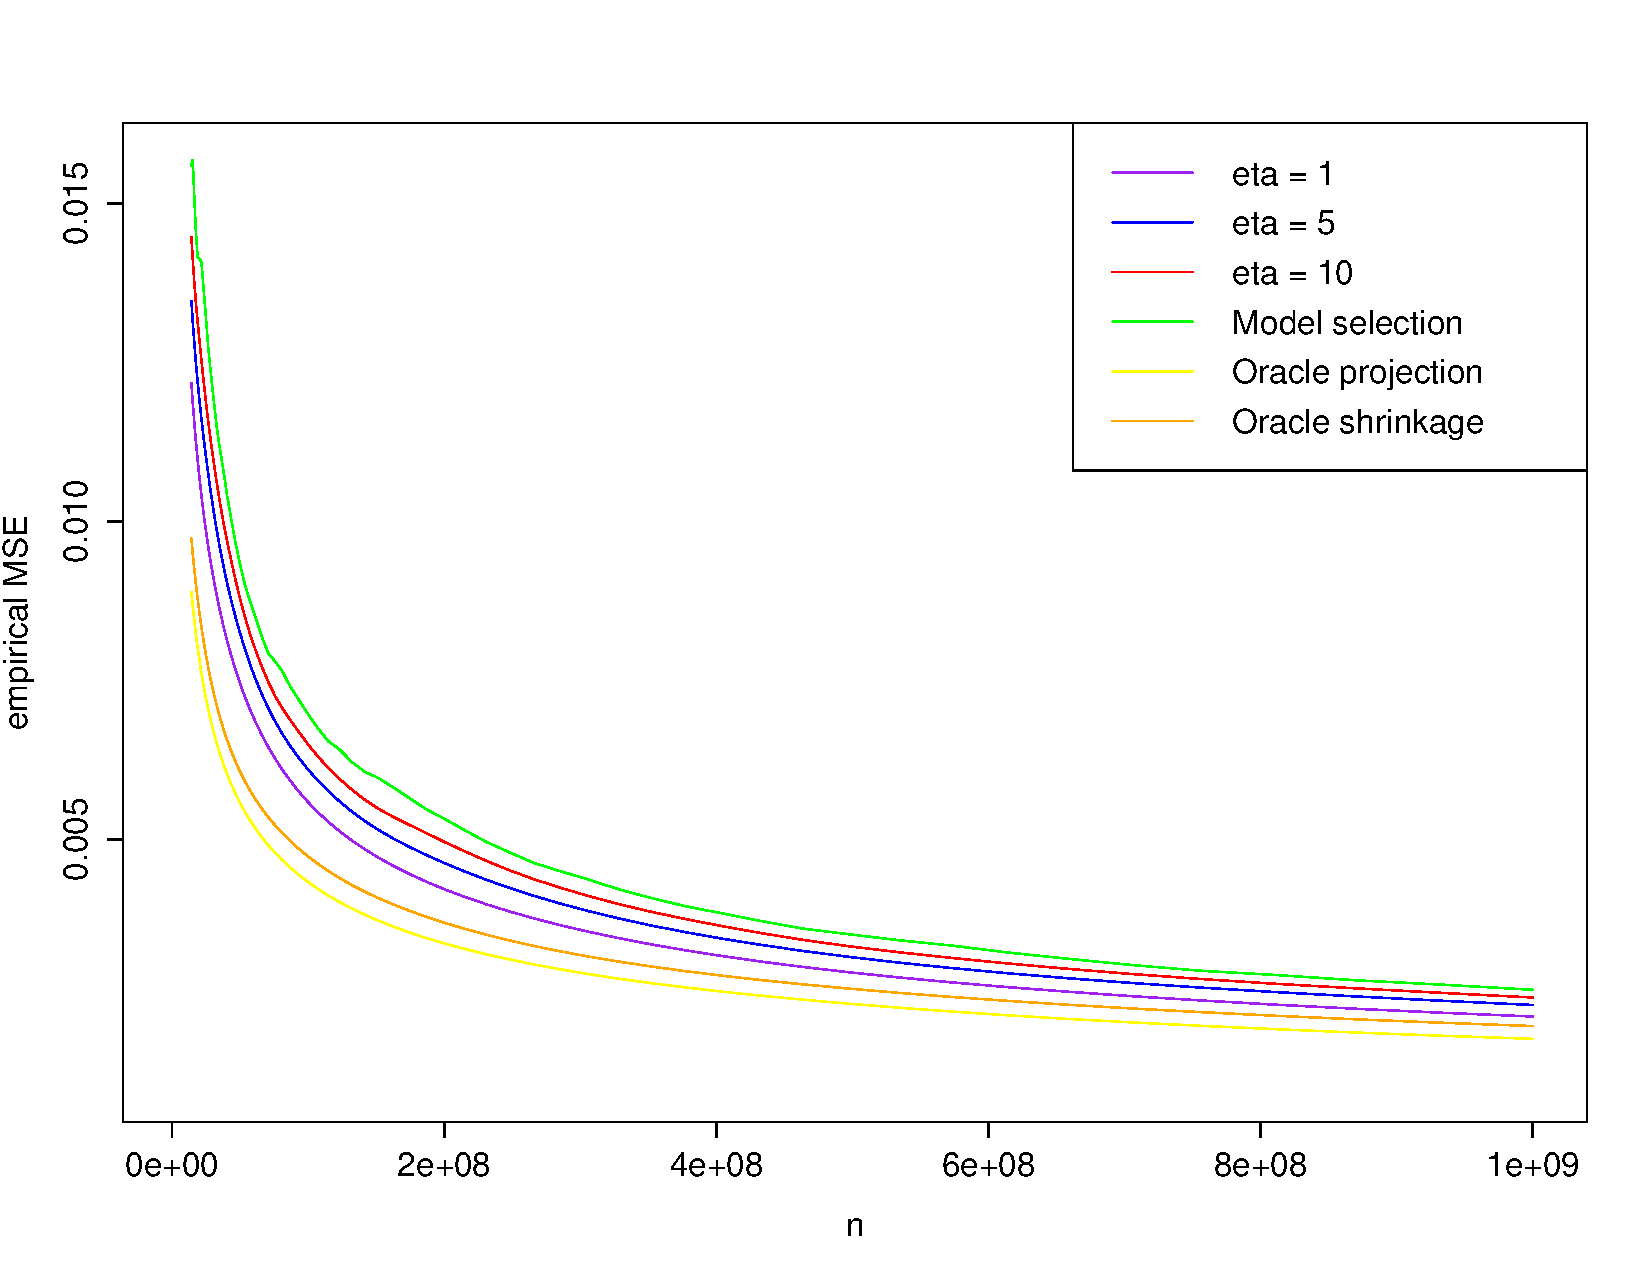
\includegraphics[width=.5\linewidth]{EQM1.pdf}
%\caption{Estimated mean of the quadratic error of the Bayes estimate for $\theta^{\circ}$ polynomial.}
%\label{EQM}
%\end{figure}
}%
%
%
\myBlock{Additional results}{%

\begin{itemize}
\item The self informative Bayes carrier is a point mass on the frequentist model selection estimate as in \cite{PM}.
\item In circular deconvolution model in presence of beta mixing data, methodology leads to oracle and minimax optimal fully data driven estimator.
\item We are currently working on an extension of this method to the real line deconvolution model.
\end{itemize}
}%
%
%
\myBlock{References}{%
	\nocite{*}%
	\bibliographystyle{abbrv}%
	\renewcommand{\section}[2]{}% HACK
	\vspace*{-7mm}% HACK
	\bibliography{myLiterature}
}%
%
%
\myBlock{Personal information}{%
	\newsavebox{\personalInformationMinipage}%
	\begin{lrbox}{\personalInformationMinipage}% Save minipage (to get size)
		\begin{minipage}[b]{0.7\textwidth}%
			\begin{itemize}[noitemsep,topsep=0pt]% ADD PERSONAL INFORMATION HERE
				\color{colBlockBodyFg}
				\item 2012-2013: BSc in Mathematics, University of Rennes 1, France
				\item 2012-2015: Master of Science (MSc) in Statistics (Dipl\^{o}me d’ing\'enieur) ENSAI - National School for Statistics and Information Analysis, Rennes, France
				\item 2013-2015: MSc in Mathematical Statistics, University of Rennes 1
				\item 2015-2018: Research assistant, Heidelberg University
				\item 2015-2018: PhD student in the RTG 1953, Heidelberg University
			\end{itemize}
		\end{minipage}%
	\end{lrbox}%
	\usebox\personalInformationMinipage% typeset minipage
	\begin{minipage}[b][\ht\personalInformationMinipage][t]{0.3\textwidth}
		\flushright
		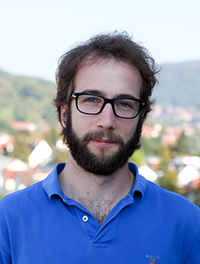
\includegraphics[width=0.5\linewidth]{test}% ADD PICTURE HERE
	\end{minipage}
}%
%
%
%
%%%%%%%%%%%%%%%%%%%%%%%%%%%%%%%%%%%%%%%%%%%%%%%%%%%%%%%%%%%%%%%%%%%%%%%%%%%%%%%%
% END RIGHT COLUMN
%%%%%%%%%%%%%%%%%%%%%%%%%%%%%%%%%%%%%%%%%%%%%%%%%%%%%%%%%%%%%%%%%%%%%%%%%%%%%%%%
%
%
%
			\\
		};
	%	
	\end{tikzpicture}
	%
\end{document}
%
%
%